% В этом шаблоне используется класс spbau-diploma. Его можно найти и, если требуется, 
% поправить в файле spbau-diploma.cls
\documentclass{spbau-diploma}

\usepackage{wasysym }
\usepackage{subfiles}
\usepackage{enumitem}

% \usepackage{titlesec}
% \newcommand{\sectionbreak}{\clearpage}

\begin{document}
% Год, город, название университета и факультета предопределены,
% но можно и поменять.
% Если англоязычная титульная страница не нужна, то ее можно просто удалить.
\filltitle{ru}{
    chair              = {Кафедра математических и информационных технологий},
    title              = {Генерация речи с учётом индивидуальных особенностей},
    % Здесь указывается тип работы. Возможные значения:
    %   coursework - Курсовая работа
    %   diploma - Диплом специалиста
    %   master - Диплом магистра
    %   bachelor - Диплом бакалавра
    type               = {master},
    position           = {студента},
    group              = 604,
    author             = {Курбанов Рауф Эльшад оглы},
    supervisorPosition = {},
    supervisor         = {Шпильман А.\,А.},
    reviewerPosition   = {},
    reviewer           = {Тузова Е.\,А.},
    chairHeadPosition  = {д.\,ф.-м.\,н., профессор},
    chairHead          = {Омельченко А.\,В.},
    % university = {САНКТ-ПЕТЕРБУРГСКИЙ АКАДЕМИЧЕСКИЙ УНИВЕРСИТЕТ},
    % faculty = {Центр высшего образования},
    % city = {Санкт-Петербург},
    % year             = {2013}
}
\filltitle{en}{
    chair              = {Department of Mathematics and Information Technology},
    title              = {Speech generation with individual characteristics},
    author             = {Rauf Kurbanov},
    supervisorPosition = {},
    supervisor         = {Alexey Shpilman},
    reviewerPosition   = {},
    reviewer           = {Ekaterina Tuzova},
    chairHeadPosition  = {professor},
    chairHead          = {Alexander Omelchenko},
}
\maketitle
\tableofcontents
% У введения нет номера главы
% \section*{Abstract}
% \subfile{sections/abstract}

\section*{Введение}
% \documentclass[../diploma.tex]{subfiles}

% \begin{document}
        
    \label{sections/introduction}
    
    В данной работе исследуется метод генерации голоса с допольнительными характеристиками.
    Главным вдохновением к проведённой работе послужили недавние продвижения в области нейросетевых  генеративных архитектур, способных генерировать такие сложные вероятностные распределения как человеческая речь\cite{article:van2016wavenet}.

    % сделай отсылки на другие секции
    
    % Мне повезло начать писать свою магстрскую работу в эпоху второго рассвета нейросетей. Благодаря дешевизне вычислительных ресурсов нейроннные сети вновь привлекли внимание исследователей и инженеров и начали создавать вокруг себя отдельную подобласть машинного обучения. Сейчас разработка архитекут нейросетей стала обособленным искусством искусством. Каждый новый приём, придуманный архитекторами нейросетей открывает возможности для новый и новый state of the art решений, привлекая инеженеров и Data Scientist'ов. 
    
    % Одним из таких новыз приёмов, в каком-то смысле давших жизнь это статье стали дырявые свёртки. Такие свёртки дают возможность строить нейронные сети, способные справиться с крупномасштабным анализом входных данных с вполне приемлимой на практите вычислительной стоимостью. Грубо говоря, о слоях дырявых свёрток можно думать как о филтрах, позволяющих пропускать учаски данных, запонимая только "полезную" информацию и охватывающих очень большой участок.
    
    % Нельзя рассказать о вдохновении к этой работе, упустив краеугольную публикацию, на основе которой и строились все наши исслодования. Вот эта публикация непосредственно перенесла идею использования дырявых свёрток к контексте генератиыных моделей в таких работах как PixelCNN[ссыль] PixelNet[сслыль]. Авторы перенесли этот опыт в контекст генерации аудио в итоге разработав новый state of the art в генерации голоса WaveNet[сслыль].
    
    % В данной работе хотелось бы раскрыть потенциаль WaveNet, уточнить вскользь описанные аспекты реализации. В полной мере утилизировать концепт локальных услових в архитектуре. Во-вторых, после того-как получим детальную открытую и протестированную реализацию, хотелось бы внести модификации в архитектуру. 
    
    % Улитимативной целью было бы исслоедовать возможности feature engineering'a для передачи в сеть в качестве локальных условий и на основе последнних решения задачу text2speech c учётм индивидуальных особенностей голоса.
    
    % В чем идея? Ну я просто заценил классную статью про wavent и решил, но заметил что там написано ну оччень мало и было бы круто как минимум заимплеменитьт эту шутку и посмотреть как она работает. Если это и правда фурычит то это просто офигенно, пушечная нейросетка и даже не рекуррентная. Но потом мне пришла в голову идея ещё и прокачать эту штуку, потому что создатели заложили возможность использовать conditioning. То есть можно подавать допольнительные условия помимо звука. Тогад я решил что былы бы круто если нейросетть будет уметь призносить текст кастомным голосом того чувака, которого я захочу. 

% \end{document}


% \subfile{sections/introduction}

\section{Мотивация}
\subfile{sections/motivation}

\section{Генеративные модели}
\subfile{sections/generative_models}

\section{Обзор решений}
\subfile{sections/existing_solutions}

\section{Wavenet}
\subfile{sections/wavenet}

\section{Задачи}
\subfile{sections/goals}

\section{WaveNet с условием}
\subfile{sections/conditional_wavenet}

\section{Датасет}
В качестве данных в данной работе использовался корпус CSTR VCTK[ссыль], размещённый в открытом доступе. Корпус CSTR VCTK включает в себя речь, произнесённую 109 нативными носителями английского языка с разнообрадными акцентами. Каждый оратор зачитывает около 400 предложений, выбранных из газет плюс специалные отрывки, подобранные чтобы подчеркнуть акцент говорящего. 

К каждой голосовой записи прилагается текст, однако текст не выровнен по аудио как если бы это были субтитры. Всё что у нас есть это набор звуковых файлов в формате \.wav с соответсвуюшим какждому .txt файлом.
Тот факт, что данные невыровнены имеет большое значение, т.к. это сильно усложнит нам задачу выравнивания признаков выделенных из текста вдоль соответсвующих участков аудио.

Продолжительность аудио варируется от 1 до 11 секунд со стандартным отклонением около секунды, что более чем достаточно для нашей задачи, т.к. генерация даже небольших звуковых файлов занимает достаточно много времени на машине, которую мы использовали для поставновки экспериментов.


\section{Реализация}
\subfile{sections/implementation}

\newpage
\section{Генерация}
\begin{figure}[h!]
  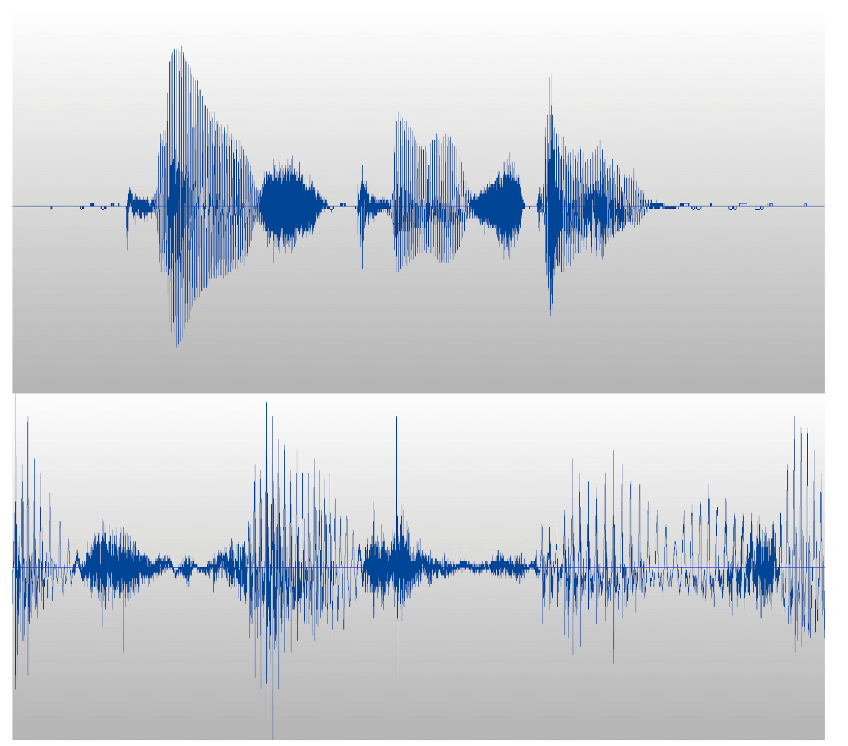
\includegraphics[scale=0.6]{img/compare}
  \caption{Сравнение сгенерированного сигнала с сигналом из обучающей выбоки}
  \label{fig:perf}
\end{figure}


% \section{Тестирование}
\newpage
\section{Feature engineering}
\subfile{sections/feature_engineering}

\section{Performance}
Время обучения растёт линейно относительно ширины сети. То есть линейно от количества признаков, которые мы передаём в локальном условии. Значит мы не можем закидывать слишком много фич, потому что нам мощности не позволяют.

\begin{figure}[h!]
  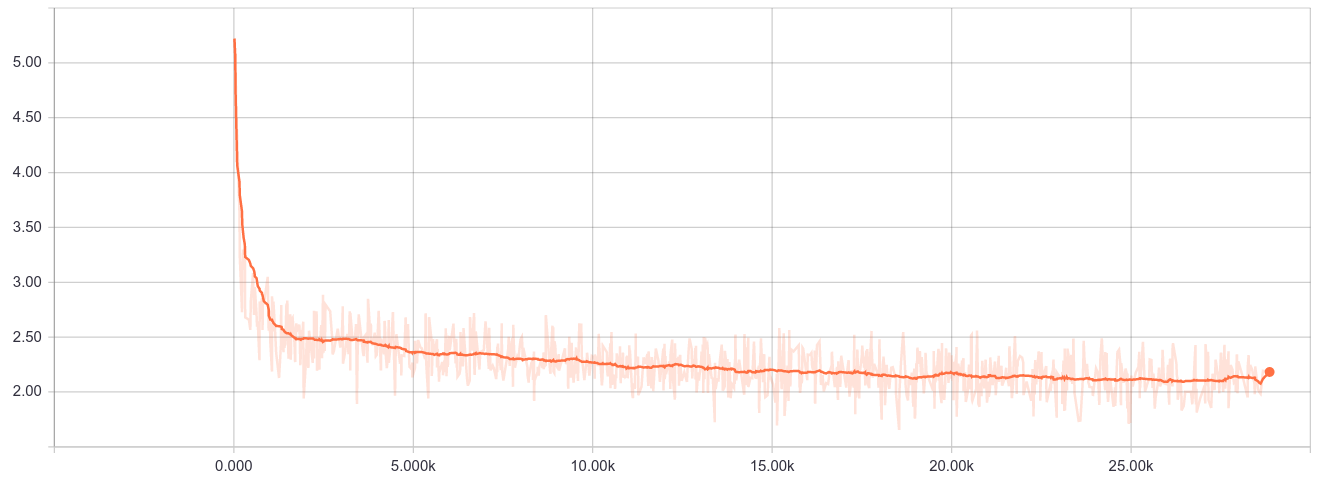
\includegraphics[scale=0.36]{img/perf}
  \caption{Изменение функции потерь в процессе обучения}
  \label{fig:perf}
\end{figure}



\section{Результаты}
На самом деле в задаче генерации трудно использовать какую-то строгую метрику для оценки качества результатоы. Да, можно в каком-то смысле считать расстояние от сгенерированного текста до настоящего, но вообще говоря сгененрировать точно такой же текст не стояло нашей задачей. Даже авторы статьи сипользовали специальную метрику.[напиши про метрику] 
\subsection{Какие-то цифры}

\bibliographystyle{ugost2008ls}
\bibliography{diploma.bib}
\end{document}
